%!TEX root = informe.tex
\chapter{Prefabricados del cemento. Adoquines}
\section{Origen del estudio}
Malaka de Prefabricados es una empresa malagueña que inició su actividad en 1994. Su compromiso consistía en integrarse en el tejido industrial de la provincia, estableciendo lazos con otras industrias locales, y apostar por un producto de calidad que marcara la diferencia en el mercado sin repercutir en el precio.

\begin{figure}[!htb]
\centering
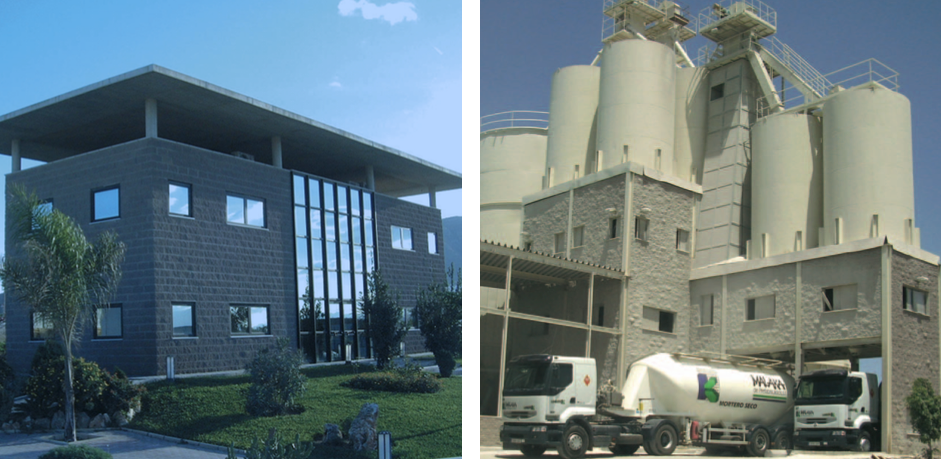
\includegraphics[width=15cm]{malaka1.png}
\caption[Instalaciones de Malaka de Prefabricados.]{Instalaciones de Malaka de Prefabricados. Fuente: \protect\cite{malakacatalogo}.}
\label{fig:malakainstalaciones1}
\end{figure}

A finales de la década de los 90 y principios del nuevo milenio experimentaron un fuerte crecimiento como consecuencia del rápido auge del sector de la construcción en Andalucía, convirtiéndose en un referente de los prefabricados en la provincia y en la comunidad autónoma.

Sus principales líneas de producción son los adoquines, bloques y bordillos de hormigón, a los que se dedica por completo una planta de producción automatizada. La línea de adoquines dispone de varias gamas de producto debido a la versatilidad y demanda de la que disfruta. El resto de productos —tubos, registros, aligerantes, casetones y mortero seco ensilado— se fabrican en la segunda planta.

\begin{figure}[!htb]
\centering
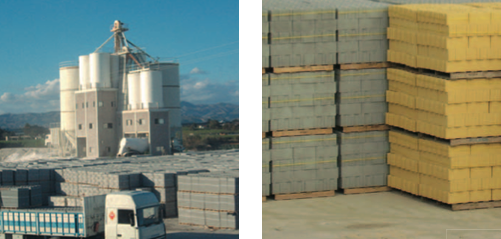
\includegraphics[width=15cm]{malaka2.png}
\caption[Instalaciones accesorias de Malaka de Prefabricados.]{Instalaciones accesorias de Malaka de Prefabricados. Fuente: \protect\cite{malakacatalogo}.}
\label{fig:malakainstalaciones2}
\end{figure}

El compromiso de calidad en sus productos pasó por cumplir todos los requisitos de la normativa española y europea, adoptando el marcado CE como sello de calidad. Tanto clientes como partners pueden dar muestra de su confianza en la calidad de los mismos. Entre sus principales proyectos se encuentran el Palacio de Deportes Martín Carpena (Ferrovial—Agroman), el Parque Temático de Melilla (Dragados) y colaboraciones con los ayuntamientos de Marbella y Estepona.

Durante los casi veinte años en la industria han intentado adoptar las mejores y más novedosas tecnologías de fabricación del sector, ampliando de forma progresiva el tamaño de sus instalaciones en la Finca Pizarro, a las afueras de la ciudad de Málaga.

La empresa adoptó a principios de 2000 la Certificación de Sistemas de Gestión de la Calidad (ISO 9001) y varios años más tarde la Certificación Sistemas de Gestión Ambiental (ISO 14000) como referente de compromiso con la calidad de su producción y con el medioambiente.

\section{Historia de los adoquines}
A lo largo de la historia de la humanidad se han ido utilizando diferentes tipos de adoquines para pavimentar los suelos urbanos. Los primeros adoquines eran de piedra, obtenidos a partir de los guijarros de río colocados sobre una capa de arena, usando una mezcla de cal y arena como sellante de juntas  \cite{euroadoquin}.

Debido al coste y el ruido del tráfico rodado, en la primera mitad del siglo XIX comenzaron a usarse los adoquines de madera, utilizando para el sellado residuos bituminosos. Su reducida duración y la posterior aparición de los neumáticos hicieron que los adoquines de madera fueran sustituidos por un modelo cerámico, con el que se usaba la misma arena tanto para la base como sellante.

Los adoquines de piedra iniciales seguían siendo más resistentes y además no eran tan deslizantes como los cerámicos. A finales del siglo XIX se fabricó por primera vez el \textbf{adoquín de hormigón}. Estos adoquines proporcionaban una mayor uniformidad que los de piedra, eran muy resistentes y con un coste inferior. Alemania y Holanda fueron los primeros en incorporar este nuevo formato de adoquín a sus núcleos urbanos. Al principio se usaban modelos que imitaban a los de piedra tanto en forma como colocación, pero pronto se añadieron formas dentadas o curvas, permitiendo una mejor alineación con el trazado.

Finalmente, durante la década de los 70 se mejoraron sustancialmente los sistemas de fabricación, permitiendo una gran variedad de modelos de adoquines y un abaratamiento de los costes de fabricación e instalación que llega hasta nuestros días.

\subsection{Ventajas del uso de adoquines}

En comparación con otros tipos de pavimentos tales como los asfálticos o los pavimentos contínuos hormigonados, los adoquines presentan las siguientes ventajas:

\begin{itemize}
\item Fabricación: no se utilizan derivados del petróleo, que suelen ser caros y contaminantes, además de requerir una mayor aportación de energía durante el proceso de fabricación. En contraposición, pueden utilizarse cementos y áridos locales, disminuyendo los costes de transporte.

El proceso de fabricación de los adoquines requiere una maquinaria específica debido a que son sometidos a presión y vibración para segurar una resistencia y durabilidad adecuadas. Esto implica un control sobre la fabricación, consistencia y fiabilidad del producto mayor que el resto de pavimentos.

\item Instalación: aunque los adoquines pueden colocarse de forma automatizada, están diseñados de base para ser colocados manualmente, permitiendo instalarse en zonas de difícil acceso, cargas elevadas (muelles de carga, aeropuertos, \ldots), resolver trazados complejos o pendientes pronunciadas. A diferencia de los pavimentos asfálticos, su ejecución no depende de la temperatura ambiente y pueden ser utilizados inmediatamente después de su finalización, lo que implica una reducción en los tiempos de ejecución de obra.

\item Comportamiento: los adoquines pueden ser diseñados para ser muy resistentes tanto a cargas verticales (distribuidas o puntuales) como a esfuerzos horizontales (aceleración-frenada, giros,\ldots). Además, soportan bien sin degradarse los vertidos de aceites y combustibles sobre el pavimento. Los niveles de ruido generados por el tráfico son similares o inferiores a otros pavimentos en ausencia de humedad y sensiblemente inferiores en condiciones de humedad, especialmente a bajas velocidades. La resistencia a deslizamiento es mayor al del resto de pavimentos.

\item Mantenimiento: la vida útil del adoquín viene determinada principalmente por el comportamiento de la base, subbase y explanada y no por el propio adoquín. La vida útil de cálculo suele ser a 30 años, aunque en condiciones normales puede superar los 50 años. De esta manera, al renovar el pavimento se pueden reutilizar entre un 90 y un 95\% de los adoquines originales \cite{euroadoquin}. El adoquín es la mejor opción en zonas donde aún no se han implantado todos los servicios de públicos debido a que pueden ser levantados fácilmente para llevar tareas de instalación o reparación en el subsuelo. La conservación de los adoquines se limita al relleno de juntas erosionadas con arena de sellado cada cierto tiempo y a la reposición de adoquines fracturados.

\item Costes: aunque inicialmente el precio del metro cuadrado instalado es algo superior a otros pavimentos, a largo plazo es mucho más barato debido al menor mantenimiento y la reutilización de piezas. Los pavimentos asfálticos y hormigonados requieren un mayor esfuerzo e inversión a la hora de ser reparados o retirados para acceder al subsuelo.

\item Aspecto estético: actualmente los adoquines pueden diseñarse de todas formas, texturas, colores y disposiciones según las necesidades de la obra.
\end{itemize}

\subsection{Desventajas del uso de adoquines}

Realmente el uso de adoquines apenas tiene inconvenientes, aunque existen varios, entre los que destacan:
\begin{itemize}
  \item Incomodidad: debido a que el pavimento está lleno de juntas de separación entre adoquines y poco a poco se vuelve irregular, la circulación y el paso pueden ser incómodos y conllevar mayores costes de operación a los vehículos.
  \item Nieve: el pavimento de adoquines suele ser irregular y no permite bien la retirada de nieve en zonas con climas donde nieva mucho. Por otro lado, la nieve se derrite antes en pavimentos de asfalto, de color negro, debido al calentamiento del sol.
\end{itemize}

\section{Materias primas}
Las características de las materias primas que se pueden emplear en la fabricación de los adoquines se contemplan en la norma UNE EN 1338:2004/AC:2006. En ella se especifican detalladamente los materiaes, propiedades, requisitos y métodos de ensayo de los adoquines prefabricados de hormigón no armados y accesorios complementarios, previstos para uso peatonal, uso en áreas sometidas a tráfico de vehículos y cubiertas, como por ejemplo: aceras, límites de áreas, sendas para bicicletas, aparcamientos, carreteras, autopistas, áreas industriales, aeropuertos, estaciones de autobuses y gasolineras. Esta norma no trata la visibilidad y la tactibilidad de los adoquines ni los adoquines permeables.

\subsection{Cemento}
El cemento es un conglomerante, formado a partir de arcilla y caliza (\ce{CaCO3}), que se endure al mezclarse con agua. Para producir cemento (ver figura \ref{fig:cemento}), la arcilla y la caliza se muelen juntas. A esta mezcla se le añade yeso para conferirle la propiedad de fraguar y endurecerse. El resultado se introduce en un horno rotatorio, normalmente seco por ser más eficiente energéticamente, a una temperatura aproximada de 1450\si{\celsius}. A continuación se introduce el material en un incinerador donde el calentamiento produce la liberación del \ce{CO2} de la caliza y se produce el cemento \emph{clinker}.

\begin{center}
\ce{CaCO3 + calor -> CaO + CO2}
\end{center}

El clinker es el óxido de calcio (\ce{CaO}) obtenido de la reacción anterior, que puede encontrarse acompañado de otros minerales como hierro, aluminio o silicio. El aporte de calor necesario para obtener el clinker representa la mayor parte del coste energético en la producción de cemento.

Por último, se produce la molienda del clinker junto yeso y otros materiales (bauxita, arena,\ldots) para mejorar sus propiedades, produciendo el cemento.

\begin{figure}[!htb]
\centering
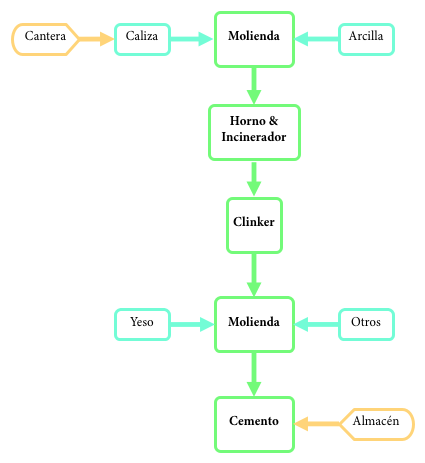
\includegraphics[width=12cm]{cemento.png}
\caption{Diagrama de flujo de la fabricación del cemento.}
\label{fig:cemento}
\end{figure}

Cuando se utiliza la palabra \emph{cemento} se refiere normalmente a un cemento tipo Portland (supone un 95\% de la producción de cementos \cite{jsjunnesson}), nombre no comercial que implica un proceso de producción y una composición característicos. De acuerdo a la norma UNE-EN 197-1:2011 \cite{une1971}, el cemento se divide en tres grupos en función de la cantidad de cemento Portland incluido: CEM I, CEM II y CEM III. El CEM I (95\% a 100\% de contenido de cemento Portland) es el más usado en la fabricación de adoquines.

Con respecto a la normativa específica de adoquines, la norma UNE 80301:1996 \cite{une80301} en el ámbito de España establece los requisitos que debe tener el cemento común. Si se utilizan cementos especiales se recurrirá a la norma UNE 80303:2013, y si son blancos a la norma UNE 80305:2012.

\subsection{Áridos}
Los áridos (entre los que se incluye la arena) son particulas de roca puede ser tanto gravas (piedras de forma natural) como macadán (piedras trituradas), teniendo cada tipo una textura diferente (figura \ref{fig:aridosnaturalesytriturados}). Se pueden añadir diferentes tamaños de áridos para ejercer una función diferente según el mismo. Fracciones menores rellenarán las cavidades que haya entre partículas mayores, aportando adherencia a costa de un mayor peso.

\begin{figure}[!htb]
\centering
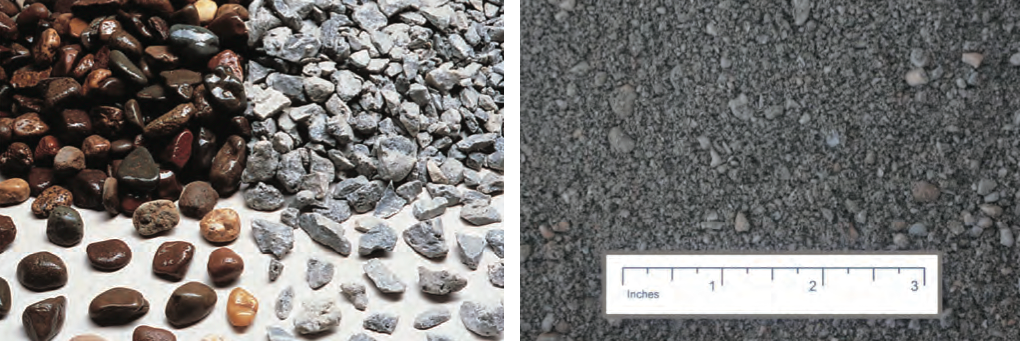
\includegraphics[width=15cm]{aridos.png}
\caption[Áridos naturales y triturados. Granulometrías.]{Áridos naturales y triturados. Granulometrías. Fuente: \cite{sustpave}.}
\label{fig:aridosnaturalesytriturados}
\end{figure}

El material de machaqueo para la producción de macadán se criba para eliminar las partículas menores. Debido a que las partículas que forman el macadán son más irregulares, es más fiable como material de relleno por su capacidad de incrustamiento (la grava tiene una forma más redondeada). El macadán se puede ser utilizado de forma más generalizada en función de la localización ya que la grava natural es un recurso más limitado.

La fuente de recursos de áridos son principalmente de río, mina o cantera o piedras trituradas (macadán). La granulometría de los áridos que se utilicen deberá cumplir las características indicada en la norma UNE EN 1338:2004/AC:2006.

\subsection{Agua}
El agua es muy importante en la constitución del hormigón. Reacciona químicamente con el cemento —hidratación— para proporcionar las propiedades deseadas del hormigón \cite{nrmca}. El agua de amasado es la cantidad de agua que toma contacto con el cemento y se usa para determinar las proporciones del resto de elementos para formar la mezcla. La fuerza y la durabilidad del cemento viene dado en gran parte por la cantidad de agua.

Además de su cantidad, la calidad del agua utilizada tiene efectos importantes en las propiedades del hormigón fresco, tales como el tiempo de fraguado y la facilidad de trabajo. También tiene importantes en la fuerza y durabilidad del hormigón endurecido.

\subsubsection{Fuentes posibles de agua}

Por norma general el agua adecuada para el consumo humano —agua potable— es válida. No obstante, el agua no potable puede ser utilizada siempre que no tenga un impacto negativo en las propiedades del hormigón. La mayoría de las plantas tienen una fuente de agua municipal que proporciona potable sin pruebas de calidad. En zonas rurales o en plantas portátiles in situ —instaladas y desinstaladas en el propio lugar del proyecto—, habrá que utilizar fuentes de agua no potable como ríos o masas de agua.

Otra fuente de agua es la reciclada de la limpieza —agua de lavado— de la mezcladora y otros elementos de la planta. También se podrá aprovechar el agua de precipitaciones atmosféricas que pueda recolectarse en las instalaciones de la planta.

El agua de procesado no sólo se genera de la fabricación del hormigón, sino también del lavado del hormigón reciclado. Los sistemas de recolección procesan el agua con el cemento y los áridos en forma de lechada que puede ser también utilizada como agua para la mezcla de hormigón.

Las normativas medioambientales suelen requerir que las plantas de fabricación traten y procesen tanto el agua de lluvia como el de procesado —agua de operaciones— para que adquiera ciertos niveles de pH y contenidos sólidos antes de que abandonen las instalaciones \cite{ermco}.

\subsubsection{Cualificación del agua no potable}
El agua es el recurso más importante para el ser humano. En algunas zonas el suministro de agua potable es muy escaso. El uso de fuentes de agua no potables para la producción de hormigón mantiene una producción sostenible de hormigón conservando los recursos de agua potable. La gestión del agua procedente de la producción de hormigón conforme con las normativas medioambientales representa un coste adicional para el fabricante, por lo que el uso de agua no potable representa un ahorro considerable en la producción de hormigón. Cuando se utilizan fuentes de agua no potable es importante verificar y documentar que las impurezas que contiene no merman las características del hormigón, ya que las fuentes pueden contener aceites, grasas, sales disueltas y otros elementos no controlados. Por esta razón, el fabricante debería tener en cuenta que su uso implica un coste adicional que evaluar y controlar.

\subsection{Aditivos}
Se podrán utilizar adiciones o aditivos siempre que produzcan el efecto deseado (acelerante, retardante,\ldots) y no afecte a las características esperadas del hormigón.
